% Copyright (c) 2008, João Henrique Ferreira de Freitas
% All rights reserved.
% 
% Redistribution and use in source and binary forms, with or without modification,
% are permitted provided that the following conditions are met:
% 
%     * Redistributions of source code must retain the above copyright notice,
%       this list of conditions and the following disclaimer.
%     * Redistributions in binary form must reproduce the above copyright notice,
%       this list of conditions and the following disclaimer in the documentation and/or 
%       other materials provided with the distribution.
%     * Neither the name of the <ORGANIZATION> nor the names of its contributors may
%       be used to endorse or promote products derived from this software without 
%       specific prior written permission.
% 
% THIS SOFTWARE IS PROVIDED BY THE COPYRIGHT HOLDERS AND CONTRIBUTORS "AS IS" AND ANY 
% EXPRESS OR IMPLIED WARRANTIES, INCLUDING, BUT NOT LIMITED TO, THE IMPLIED WARRANTIES
% OF MERCHANTABILITY AND FITNESS FOR A PARTICULAR PURPOSE ARE DISCLAIMED. IN NO EVENT
% SHALL THE COPYRIGHT OWNER OR CONTRIBUTORS BE LIABLE FOR ANY DIRECT, INDIRECT, INCIDENTAL,
% SPECIAL, EXEMPLARY, OR CONSEQUENTIAL DAMAGES (INCLUDING, BUT NOT LIMITED TO, PROCUREMENT
% OF SUBSTITUTE GOODS OR SERVICES; LOSS OF USE, DATA, OR PROFITS; OR BUSINESS INTERRUPTION)
% HOWEVER CAUSED AND ON ANY THEORY OF LIABILITY, WHETHER IN CONTRACT, STRICT LIABILITY,
% OR TORT (INCLUDING NEGLIGENCE OR OTHERWISE) ARISING IN ANY WAY OUT OF THE USE OF THIS
% SOFTWARE, EVEN IF ADVISED OF THE POSSIBILITY OF SUCH DAMAGE.
% 
% $Id$

\section{Resultados e Discussão} \label{sec:resultados} \label{subsec:sobre}

A taxionomia (vide anexo \ref{sec:anexob}) realizada inicialmente foi deixada em segundo plano, na forma de consulta sempre que dúvidas relacionado aos artefatos do projeto surgiram. Uma espécie de guia de consulta rápida onde foi possível determinar as próximas ações para determinada atividade como por exemplo testes de regresão, submissão de patch, padrões de codificação e design.

Antes de iniciarmos a discussão da experiência, é necessário posicionar o leitor nos recursos desejados e implementados no projeto de SL/CA escolhido anteriormente. Em resumo a funcionalidade desejada (vide anexo \ref{sec:anexoa}) era o suporte a uma camada de abstração no software de gerenciamento de backups de rede \textit{Bacula}. Antes do nosso patch (denomidado \patch ou simplesmente \patchshort), o software Bacula contava apenas com o suporte a SGBDs livres (Mysql, Postgresql e SQLite) nos quais eram implementados nativamente, via APIs (Application Programming Interface ou Interface de Programação de Aplicativos) padrões para acesso aos SGBDs específico, no código do Bacula. 

A implementação de uma camada de abstração possibilitou a integração com outros SGBDs livres ou proprietários (vide anexo \ref{sec:anexod}) sem mudanças no código do Bacula, ou com mudanças mínimas.\footnote{Na realidade, como há diversos dialetos para a linguagem SQL implementada nos SGBDs, torna-se necessário revisar as consultas utilizadas pelo Bacula antes do mesmo suportar oficialmente outro SGBD.} Além de possibilitar um único ponto de manutenção para o código referente ao interfaceamento com SGBDs. Nas seções seguintes, apresentamos os detalhes da implementação e também o modelo de desenvolvimento utilizado.

\subsection{Implementação do patch} \label{sec:anexoe}

O software Bacula é um conjunto de softwares (vide figura \ref{fig:arqbacula}) no qual permitem gerenciar \textit{backups}, \textit{restores} e verificações através da rede de diversos tipos de computadores. Bacula é relativamente fácil de usar e eficiente, oferece muitos meios de armazenar os dados e recursos para gerenciá-los, procurá-los e recuperá-los. A maioria do código fonte está licenciada sob a licença GPL versão 2 e com direitos passados para a Free Software Foundation Europa.

Como podemos notar na figura \ref{fig:arqbacula} o software Bacula possui um conjunto de programas nos quais podem ser instalados e executados em diferentes máquinas dentro de uma rede.
Os principais componentes são:
\begin{itemize}
\item Servidor de Backup, denominado de \textit{bacula-dir}, com as funções de orquestrar toda a solução;
\item Servidor de Armazenamento, denominado de \textit{bacula-sd}, responsável por armazenar todos os arquivos enviados pelos bacula-fd;
\item Servidor de Arquivos, denomindado de \textit{bacula-fd}, responsável por enviar para o bacula-sd os arquivos necessários para serem armazenados provenientes dos computadores de uma rede;
\item Estações de Administração, denomindas de \textit{console}, são utilizadas para controlar via linha de comando ou interface gráfica as operações e tarefas do Bacula;
\item Servidor de Banco de Dados, denominado \textit{catalog database} ou banco de dados, armazena os meta-dados (características de cada arquivo).
\end{itemize}

\begin{figure}[h]
 \centering
 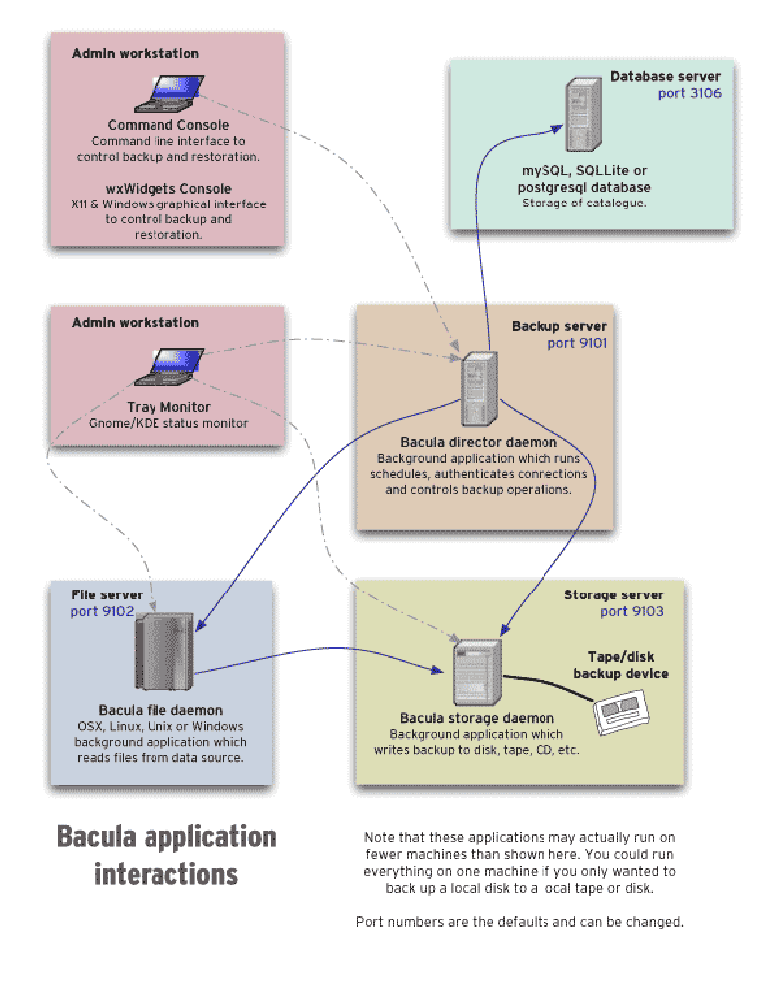
\includegraphics[scale=0.8]{../../doc/figuras/bacula-applications.eps}
 % bacula-applications.png: 1179666x1179666 pixel, 0dpi, infxinf cm, bb=
 \caption[Arquitetura geral do Bacula]{Arquitetura geral do sistema \\ \url{http://www.bacula.org/en/dev-manual/What_is_Bacula.html}}
 \label{fig:arqbacula}
\end{figure}

Durante a implementação do patch \patchshort, concentramos apenas nos componentes bacula-dir e catalog database. Não tivemos a necessidade de interferir nos outros componentes do sistema pois tratavam operações nas quais não nos interessavam no momento.

Para ajudar no entendimento, as figuras \ref{fig:unico} e \ref{fig:dbi} oferecem uma visão geral antes e depois da implementação do patch. 

Na figura \ref{fig:unico} notamos a utilização de um único banco de dados por binário, ou seja, a escolha de qual banco de dados utilizado é definida durante a compilação do código fonte do Bacula, no qual eram definidos os códigos necessários para construir o driver de acesso nativo via API própria de cada banco de dados. A camada sql\_$\ast$.c utiliza as funções definidas em [banco de dados].c,  onde [banco de dados] pode ser apenas um dentre: mysql, postgresql, sqlite. Desta forma, uma vez compilado, o usuário apenas utilizaria o banco de dados escolhido. 
Um outro ponto é o suporte aos bancos de dados limitados, ou seja, apenas para os SGBDs codificados no Bacula.

Já na figura \ref{fig:dbi} observamos um novo cenário no qual uma camada de abstração (via biblioteca libdbi) e um driver (dbi.c) para fazer a interface entre a camada sql\_$\ast$.c e a libdbi foi implementado. Basicamente para garantir dois pontos: 
\begin{itemize}
\item O primeiro é a independência do banco de dados a ser utilizado pelo Bacula. 
\item O segundo ponto é a possibilidade de utilizar vários tipos de SGBDs para armazenar meta-dados de arquivos.                                                                   \end{itemize}
Um exemplo do segundo ponto abordado é a possibilidade de realizar backups entre bancos de dados ou até mesmo a transferência de um catálogo de um banco de dados para outro completamente distinto em caso de problemas ou manutenções.

\begin{figure*}[h]
 \centerline{
  \subfigure[Único banco de dados por binário]{
  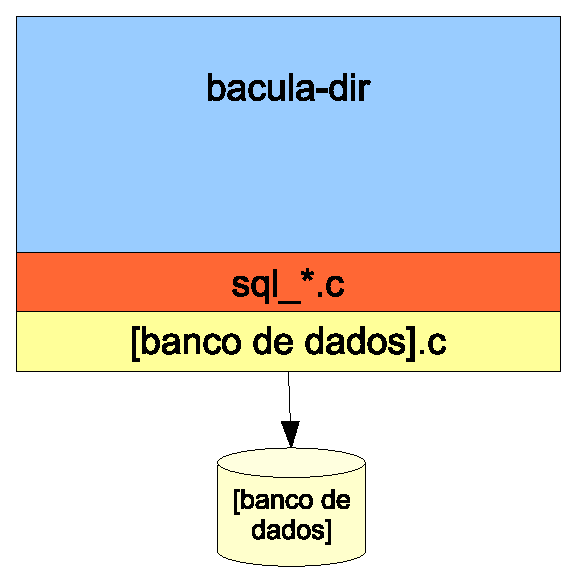
\includegraphics[width=5cm]{../../doc/diagramas/bacula-dir-sgbd.eps}
  \label{fig:unico}
  }
  \hfil
  \subfigure[Vários tipos de banco de dados por binário]{
  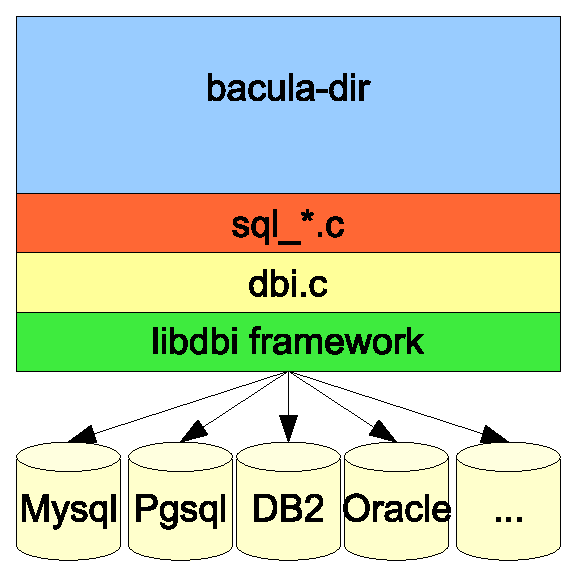
\includegraphics[width=5cm]{../../doc/diagramas/bacula-dir-dbi.eps}
  \label{fig:dbi}
  }
  \label{fig:comparativo}
 }  
 \caption[Comparativo de implementação]{Comparativo da implementação realizada \subref{fig:unico} e \subref{fig:dbi}}
\end{figure*}

\subsubsection{Limitações}

A principal limitação encontrada foi referente a existência de diversos tipos de SGBDs utilizando diferentes dialetos e recursos da linguagem SQL. Não é possível prever todos os casos. Há consultas que funcionam em todos os SGBDs e outras que são específicas e devem ser tratadas a parte. 

A biblioteca libdbi oferece uma abstração para os diferentes tipos de APIs de cada fabricante de SGBDs mas a mesma não oferece nenhum suporte aos diferentes tipos de SQL utilizados por eles.

Sendo assim o Bacula deve ser preparado para suportar os diferentes dialetos SQL, ou seja, para cada banco de dados temos um conjunto de SQL que devem ser adptadas e suportadas para que o SGBD seja efetivamente suportado. Isso se torna uma limitação pois necessita de uma intervenção no código para o correto funcionamento.

\subsubsection{Implementação}

As tarefas de criação do ambiente necessário para a implementação e definição de quais arquivos seriam necessários criar ou alterar não foram complicadas. Notamos um software bem modularizado e dividido para facilitar a manutenção e adiçaõ de novos recursos. A seguir apresentamos uma macro lista dos itens no qual foram necessário trabalhar:

\begin{itemize}
\item Alteração no arquivo \url{src/cats/cats.h}: 
 \subitem inclusão da regra de compilação condicional HAVE\_DBI para o compilador reconhecer o código para o driver DBI
 \subitem adaptado a estrutura de dados B\_DB, responsável pelo gerenciamento de todos os itentes relacionados a banco de dados, dentro do Bacula, bem como as definições de várias funções para a API da libdbi
\item Alteração dos arquivos \url{src/cats/sql*.c}: incluindo a regra de compilação condicional HAVE\_DBI
\item Criado o arquivo \url{src/cats/dbi.c} baseado no código \url{src/cats/postgresql.c}
 \subitem tranformado e convertigo as funções presentes no arquivo src/cats/dbi.c de um código com APIs referentes ao SGBD postgresql para APIs da  biblioteca DBI. Evidente que muitas funções presentes no SGBD postgresql não seguiam a mesma lógica utilizada na biblioteca DBI. Sendo necessário estudar as documentações e códigos de ambas para entender o funcionamento e decidir se a API da biblioteca DBI atendia ou não a forma na qual o Bacula estava projetado para interagir com um SGBD. 
\item Alterado o arquivo \url{src/dird/dird_conf.h} e \url{src/dird/dird_conf.c}
 \subitem adicionado a opção de configuração dbdriver no qual informava ao Bacula qual driver e banco de dados será utilizado.
\item Alterado os arquivos \url{src/autoconf/config.h.in} e \url{src/autoconf/bacula-macros/db.m4} referentes a geração do script de autoconfiguração para compilação, baseados nas disponibilidades dos requisitos da plataforma.
\item Adaptação de todos os testes de regressão para incluir as opções de configuração para o driver DBI
\end{itemize}

\subsection{Modelo de desenvolvimento utilizado durante o experimento} 

Durante toda a experiência, como não tinhamos muito bem definido os requisitos necessários para a implementação. E tão pouco um conhecimento suficiente grande do código em que iriamos modificar, foi necessário utilizar um modelo de desenvolvimento no qual fosse permitido definir um mínimo de objetivos e logo iniciar o ciclo de desenvolvimento, após uma fase de \textit{Exploração Arquitetural} (EA). 

Atrelando ao fato de que o projeto Bacula estabelece frameworks de testes e recomendações explícitas para a utilização sempre após qualquer alteração no código fonte, e tendo em consideração que uma das premissas para a utilização do modelo em vista era uma forma de validação da implementação rapidamente para que nada fosse alterado de forma a quebrar as outras funcionalidade existentes. Achamos pertinente utilizar o modelo de \textit{Programação ou Desenvolvimento Exploratório} (vide figura \ref{fig:exploratoria}). 

Em \cite[página 31]{engenharia1} define como sendo: \textit{``O modelo de programação ou desenvolvimento exploratório visa a construção da primeira versão do sistema o mais rápido possível. Sistemas desenvolvidos assim caracterizam-se por não terem o escopo claramente definido... Após o desenvolvimento de cada uma das versões do sistema, ele é mostrado aos usuários para comentários. Modificações sucessivas são feitas no sistema até que o mesmo seja considerado adequado''}.

\begin{figure}[h]
 \centering
 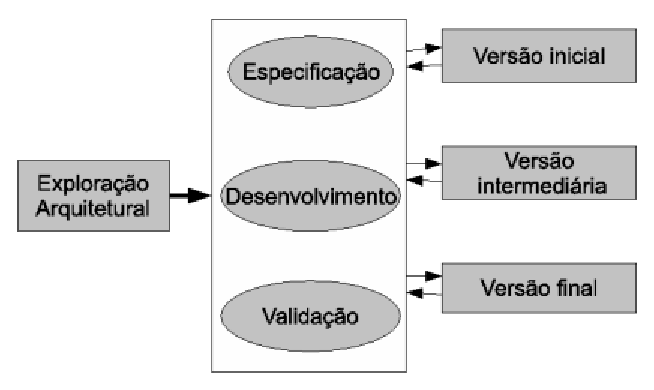
\includegraphics{../../doc/diagramas/programacao_exploratoria.eps}
 % programacao_exploratoria.eps: 1179666x1179666 pixel, 300dpi, 9987.84x9987.84 cm, bb=14 14 312 185
 \caption[Programação exploratória]{Modelo de programação exploratória \cite{engenharia1}}
 \label{fig:exploratoria}
\end{figure}

Acreditamos que não havendo um framework de testes, no qual realizamos diversos testes de regressão no projeto, não seriamos capazes de implementar as modificações propostas. Devido as chances de quebrar toda a consistência dos dados do software. Do ponto de vista do desenvolvedor, testes automáticos encorajam o desenvolvimento e aumentam o processo de \textit{refactoring}\footnote{Processo de constantes melhorias no design e código do software} \cite[página 203]{producing}.

% Exploratory programming is an important part of the software engineering cycle: when a domain is not very well understood or open-ended, or it's not clear what algorithms and data structures might be needed for an implementation, it's useful to be able to interactively develop and debug a program without having to go through the usual constraints of the edit-compile-run-debug cycle.
%  
% "Automated testing"
%
% TODO: Elaborar um texto de introdução

\subsubsection{Exploração Arquitetural e Escopo}\label{subsec:arquiterual}\label{subsec:experiencia}

%\textit{Como planejar os melhoramento e qual a melhor forma de planeja-los?}\\
Após a elaboração da classificação, de acordo com o anexo \ref{sec:anexob}, iniciamos os experimentos elaborando os requisitos necessários (vide anexo \ref{sec:anexoa:baculalibdbi}) para as melhorias objetivadas para o projeto.

Basicamente tentamos responder os seguintes questionamentos: \textit{O que?}, realmente precisamos desta funcionalidade; \textit{Porque?}, quais os fundamentos técnicos e benefícios para o projeto implementando esta funcionalidade; \textit{Como?}, quais os artefatos necessários e como implementá-los (vide anexo \ref{sec:anexoa:featurereq}). Evidente que para a última questão um conhecimento maior sobre o software em si foi necessário antes de aventurarmos em sugestionar mudanças para a comunidade do projeto. Entretanto a dificuldade relacionada em argumentar como a nova funcionalidade desenvolvida se encaixou no software foi minimizada via uma \textit{Exploração Arquitetural}, demonstrada adiante.

A melhor definição de Exploração Arquitetural (EA) é encontrada dentro do modelo de desenvolvimento XP no qual também possui uma fase exploratória e pode ser definido, segundo \cite[página 36]{procdesenv}: \textit{``A fase de exploração é anterior à construção do sistema. Nela, investigações de possíveis soluções são feitas e verifica-se a viabilidade de tais soluções... Os clientes são consultados e trazidos para dentro da equipe... Os programadores são responsáveis por fazer experimentos com a possível tecnologia e infra-estrutura a ser escolhida...''}. No contexto do trabalho, entendemos que ``clientes'' são os desenvolvedores do núcleo do projeto com uma visão mais crítica das modificações propostas e ``programadores'' são os contribuidores do patch. Asssim a visão do XP se encaixa perfeitamente para a experiência.

% Explicar melhor oque foi feito com a Exp. Arq. fazendo ref. para os emails e testes realizados anteritormente
% É a hora de usar a taxocomia em busca de informaçòes de como fazer. Relatar a procura no svn, emails antigos, guias de referencias, comunicação com outros projeto

Enfim, a Exploração Arquitetural possibilitou as atividades abaixo relacionadas e um conhecimento maior sobre o projeto de SL/CA e sua engenharia. 
\begin{description}
\item [Testar as possibilidades] ponto em que o desenvolver percebe o mal funcionamento, necessidade de manutenção ou implementação de uma nova funcionalidade.
\item [Documentar as necessidades] para levantamento e descrição dos requisitos, escopo inicial e analise de como fazer a modificação (vide anexo \ref{sec:anexoa}).
\item [Levantar feedback dos desenvolvedores] abrindo discuções formalmente, via lista de discussão ou email privado com os desenvolvedores. É importante nesta fase a argumentação técnica das modificações a serem realizadas e evidenciar os benefícios para o projeto. Muitas vezes é a partir deste ponto que a modificação pode ou não dar certo (vide anexo \ref{sec:anexod})
\item [Iniciar experimentações]: implementação dos requitisos e testes. Neste ponto os testes são fundamentais pois as novas funções ou modificações não devem quebrar o código já existente.
\item [Analisar possibilidades]: ponto em que o desenvolvedor envia os patches para aprovação pelos desenvolvedores oficiais do projeto e recebe os maiores feedbacks sobre seu trabalho.   \end{description}

É importante ressaltar que as fases \textit{Documentar as necessidades} e \textit{Levantar feedback dos desenvolvedores}, na experiência, ocorreram quase que concomitantemente devido a necessidade de saber a viabilidade da implementação para não precisar abortar os trabalhos ou se tornar inviável devido alguma barreira (vide discussões no anexo \ref{sec:anexod} para maiores detalhes).

Mesmo que o contribuidor não conheça a fundo o projeto objetivado, através da EA ele poderá se sentir confortável, ou seja, saber como e onde os artefatos do projeto se encaixam e manter um diálogo saudável com a comunidade de desenvolvedores, para realizar as implementações necessárias.
% Caminho 1: Oque deseja implementar pode estar na árvore de código do projeto. Você pode consultar o repositório em busca de logs de alterações. Geralmente as alterações são atômicas para determinados requisitos, ou seja, aparecem por inteiro provenientes de um desenvolvedor.

% Exploração arquitetural e técnica
%     Levantamento de informações relacionadas ao projeto em questão;% 
%     Necessidade de conhecer o projeto e sua engenharia pois cada um possue suas particularidades.
% 
%     Alguns detalhes importantes:
% 
%     * políticas de release
%     * documentação
%     * padrões de desenvolvimento
% 
%  
% 
%     Modelo sugerido
% 
%  
% 
%                |-----------\  |--------\    |--------------\     |--------------\ 
%        exploração          \           \                   \                    \ 
%                            analise     \                   \                    \ 
%                                       projeto              \                    \ 
%                                                          desenvolvimento        \
%                                                                               testes
% 
%                |------------------------------------||---------------------------------------|
% 
%                       foco do trabalho                            anexo do trabalho
% 
%  
% 

\subsection{Ciclo de desenvolvimento}

Após o período necessário para entendimento do projeto Bacula, iniciamos as primeiras experiências na implementação do patch. Já havíamos traçado os planos em discussões com desenvolvedores de quais arquivos seriam necessários trabalhar e os pontos de maior cautela.

\subsubsection{Padrões de projetos identificados}

Basicamente o Bacula é um software multiplataforma escrito em C/C++ com um design e codificação muito claros, bem estruturado e modular. O entendimento do código fonte não foi um problema por dois motivos: 
\begin{enumerate}
\item O projeto possue um documento de guias gerais de implementação (vide anexo \ref{sec:anexob}) no qual foi fundamental para o entendimento de diversos pontos relacionado aos padrões de desenvolvimento e arquitetura;
\item Por se tratar de uma codificação modular tinhamos a oportunidade de ler o código mais claramente e buscar rapidamente a função ou parte do código que tinhamos a necessidade de entender.
\end{enumerate}
Durante o desenvolvimento utilizamos a biblioteca (ou framework) libdbi\footnote{\url{http://libdbi.sourceforge.net/}} (vide anexo \ref{sec:anexog}), no qual permitiu o acesso aos diversos SGBDs. O ponto de maior dificuldade foram as experiências necessárias para saber como a biblioteca libdbi funcionava e como integrá-la ao projeto da melhor forma possível, ou seja, utilizando as estruturas de dados e técnicas semelhante aos \textit{drivers} já implementados, no Bacula, para acesso aos bancos de dados nativamente. Assim, grande parte do tempo foi dedicado a esta integração. 

\subsubsection{Ferramentas utilizadas}

Diversas ferramentas deram suporte às atividades ao longo do projeto e podem ser divididas em três grupos: 
\begin{itemize}
 \item Gerênciais: utilização da ferramenta \textit{dotProject}\footnote{\url{http://www.dotproject.net/}} no qual funcionou como gerenciador do projeto e controle de horas gastas;
 \item Técnicas: \textit{subversion}, para gerenciamento do código fonte; \textit{eclipse} com plugin para C/C++, utilizado como IDE e navegação no código fonte; \textit{ddd}\footnote{\url{http://www.gnu.org/software/ddd/}}, para debug do código; \textit{valgrind}\footnote{\url{http://www.valgrind.org}}, para profiling de memória e deteção de vazamentos de memória;
 \item Operacionais: bancos de dados Postgresql e Mysql; sistema operacional Ubuntu Linux 7.10.
\end{itemize}

\subsubsection{Dia a dia de trabalho}
O período de desenvolvimento pôde ser dividido nas atividades de implementação, testes, análise, discussão de problemas e submissão do patch. A figura \ref{fig:resolucao_problemas} ilustra o relacionamento entre cada atividade. 
\begin{figure}[h]
 \centering
 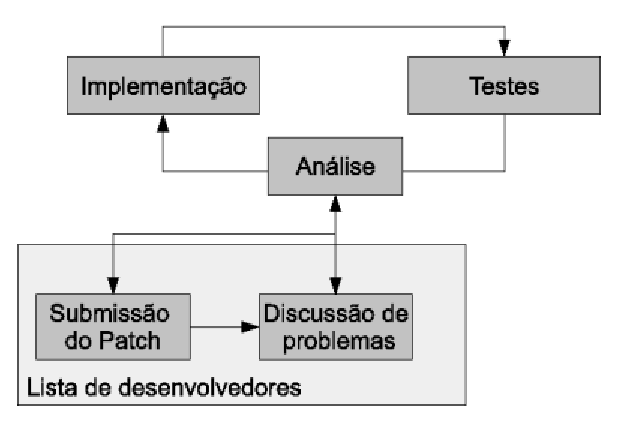
\includegraphics{../../doc/diagramas/resolucao_problemas.eps}
 % resolucao_problemas.eps: 1179666x1179666 pixel, 300dpi, 9987.84x9987.84 cm, bb=0 0 431 287
 \caption[Fase de desenvolvimento]{Fase de desenvolvimento utilizada na experimentação}
 \label{fig:resolucao_problemas}
\end{figure}

Podemos identificar que as atividades de implementação, testes e análise ocorreram de forma circular, ou seja, a cada implementação foi seguida por testes e anaĺise dos resultados. Havendo problemas ou dúvidas; eram reportadas via lista de discussão, voltando para o ciclo de implementação e verificando se os problemas reportados na lista de desenvolvimento foram sanados. Todo o ciclo se repetiu até que a implementação do patch \patchshort fosse validada, testada e integrada no repositório do projeto Bacula.

Trabalhando desta maneira, conseguimos fazer com que os desenvolvedores sugestionassem e mudassem o design caso houvesse necessidade (vide anexo \ref{sec:anexod:problemas} para mais detalhes). 

Abaixo descrevemos as atividades:

\begin{description}
\item[Implementação]: tarefas relacionadas à codificação, experimentações e sincronização com o ramo principal de desenvolvimento do projeto. As sincronizações são necessárias sempre antes de iniciar os trabalhos para verificar se nada mudou em outras partes do código fonte.
\item[Testes]: a cada codificação os testes de regressão (ou quaisquer outros) devem ser executados.
\item[Análise]: basicamente é a verificação dos testes e problemas encontrados na implementação. Caso ocorra dificuldade tais como: mudanças extremas em várias partes do código, dúvidas referentes ao design do software, mudanças de conceitos, é necessário entrar em contato com os desenvolvedores e expor os problemas encontrados.
\item[Discussão]: as necessidades especiais e problemas devem ser expostas afim de coletar feedback do trabalho e também sanar os problemas, como por exemplo: mudança de design, alteração de nomes, modificação de técnicas.
\item[Submissão]: durante a fase de análise, caso identifiquemos que o patch esta suficientemente maduro para ser submetido ou queremos demonstrar o status do trabalho, devemos submete-lo na lista de desenvolvimento para algum outro desenvolvedor possa testar, revisar e possivelmente integrar na árvore principal de código fonte do projeto.
\end{description}

\subsubsection{Submissão do patch}

Após o período de desenvolvimento, no qual não foi finalizado até a execução satisfatória de todos os testes de regressão do projeto Bacula, o patch \patchshort foi submetido na lista de desenvolvimento. Na tabela \ref{Timeline} podemos notar a relação entre a duração da fase de EA e Desenvolvimento, a submissão do patch na lista de desenvolvedores e a integração do código submetido no repositório de controle de versão. 

\begin{table}[h]
\begin{tabular}{|l|c|c|c|c|}
\hline
 & \textbf{Data} & \textbf{Submissões} & \textbf{Data Integração} & \textbf{Revision} \\ \hline
\multicolumn{ 1}{|c|}{\textbf{Exploração Arquitetural}} & 2007-12-07 &  &  &  \\ \cline{ 2- 5}
\multicolumn{ 1}{|l|}{} & 2008-01-11 &  &  &  \\ \hline
\multicolumn{ 1}{|c|}{\textbf{Desenvolvimento}} & 2008-01-18 &  &  &  \\ \cline{ 2- 5}
\multicolumn{ 1}{|l|}{} &  & 2008-02-01 & 2008-02-02 & 6358 \\ \cline{ 2- 5}
\multicolumn{ 1}{|l|}{} &  & 2008-02-12 & 2008-02-13 & 6413 \\ \cline{ 2- 5}
\multicolumn{ 1}{|l|}{} &  & 2008-02-19 & 2008-02-22 & 6464 \\ \cline{ 2- 5}
\multicolumn{ 1}{|l|}{} &  & 2008-02-21 & 2008-02-27 & 6498 \\ \cline{ 2- 5}
\multicolumn{ 1}{|l|}{} &  & 2008-02-25 & 2008-04-15 & 6825 \\ \cline{ 2- 5}
\multicolumn{ 1}{|l|}{} &  & 2008-03-17 & 2008-04-15 & 6826 \\ \cline{ 2- 5}
\multicolumn{ 1}{|l|}{} &  & 2008-04-09 & 2008-04-09 & 6817 \\ \cline{ 2- 5}
\multicolumn{ 1}{|l|}{} &  & 2008-04-14 & 2008-04-15 & 6818 \\ \cline{ 2- 5}
\multicolumn{ 1}{|l|}{} &  & 2008-04-27 & 2008-04-27 & 6874 \\ \cline{ 2- 5}
\multicolumn{ 1}{|l|}{} & 2008-05-02 &  &  &  \\ \hline
 &  &  &  &  \\ \hline
 & \textbf{Orçadas} & \textbf{Trabalhadas} &  &  \\ \hline
\textbf{Exploração Arquitetural:} & 64h & 59.89h &  &  \\ \hline
\textbf{Desenvolvimento:} & 168h & 118h &  &  \\ \hline
\end{tabular}
\caption{Timeline}
\label{Timeline}
\end{table}

Mediante as regras de licenciamento do projeto, de acordo com anexo \ref{sec:anexoc}, o patch só pôde ser aceito e integrado no repositório do projeto após o envio por carta convencional contendo a doação formalmente do código escrito para o projeto. Segundo os desenvolvedores esta é uma medida de proteção para evitar problemas legais referentes a patentes de software. 
Após o recebimento\footnote{A carta foi destinada a \textit{Free Software Foundation Europa} (\url{http://www.fsfeurope.org/}) mais especificadamente para o projeto conhecido como \textit{Freedom Task Force} (\url{http://www.fsfeurope.org/projects/ftf/about.pt.html})} da carta, o código pôde ser integrado.

Identificamos três tipos de submissões ao longo do processo de desenvolvimentos:

\begin{description}
\item[Submissão temporal] ocorreu quando houveram algumas necessidades: mostrar o status do trabalho para os desenvolvedores do núcleo, integrar código no repositório principal do projeto para testes, levantar feedback técnico a respeito da implementação (vide anexo \ref{sec:anexod:submissaotemporal}).
\item[Submissão de finalização] após a implementação, execução de todos os testes de regressão e limpeza no código fonte. Foi feita a submissão final para integração no repositório (vide anexo \ref{sec:anexod:submissaofinal}).
\item[Submissão de manutenção] consequentemente o patch \patchshort se tornou oficial e entrou num período de manutenção. Neste período podem ocorrer manutenção e melhoramentos no código, gerando submissões de manutenção (vide anexo \ref{sec:anexod:submissaomanutencao}).
\end{description}

É importante notar que não foi dado permissões de integração do código diretamente no repositório do projeto, mesmo após o envio da referida carta. Acreditamos que a razão foi a codificação de uma melhoria específica e ser a primeira vez que temos contato com o projeto Bacula.

\subsection{Exposição dos resultados}

No contexto da experiência realizada, após cinco meses de pesquisas, interações com  comunidades e desenvoldores para a resolução de todos os obstáculos técnicos encontrados, conseguimos estabilizar o patch \patchshort para integrá-lo em uma versão estável do projeto Bacula. Completando assim nossos objetivos de contribuir e capturar o processo de implementação de um patch dentro da comunidade de SL/CA. 

Na seção \ref{sec:objetivos} colocamos algumas questões inicialmente levantadas antes de iniciarmos os experimentos acima discutidos. Com o auxílio dos experimentos realizados, responderemos cada pergunta de maneira a expor as recomendações, evidenciadas nesta experiência, para futuros contribuidores em projetos de SL/CA:

\textit{Quais os caminhos e possibilidades para usuários colaborarem?} Dentre os itens comumente citados para usuários colaborarem, tais como implementação de código, testes, documentações, tradução, entre outros. Projetos de SL/CA são carentes em contribuidores que possam ajudar a definir melhores processos de desenvolvimento dentro da engenharia de software tradicional. Definir melhor não significa que os processos não existam mas sim corrigir a forma nas quais as atividades e processos ocorrem. Por exemplo: sentimos dificuldades em descobrir e verificar o status das tarefas nas quais os desenvolvedores do núcleo estavam realizando.

\textit{Como colaborar efetivamente?} A efetividade em projetos de SL/CA está ligado ao nível de conhecimento que o contribuidor possui. Por exemplo: caso ele tenha conhecimentos avançados em uma determinada linguagem de programação, é mais fácil para ele implementar códigos mais ousados, eficientes e seguros. Felizmente não é necessário possuir grandes conhecimentos para iniciar as atividades de contribuição. Numa vertente não técnica: comunicar-se e descobrir o processo utilizado pela comunidade de SL/CA e na vertente técnica analisar e entender o código fonte em busca de reaproveitamento, modularidade e averiguando como implementar o necessário sem quebrar a consistência e padronização do projeto.

% Conlusão 1: O desenvolvedor que se aventura em projetos SL/CA necessita ter uma carga de conhecimentos muito bem estruturada em portabilidade e linguagens de programação.
% 
% Conclusão 2: Analisar o código fonte em busca de reaproveitamento de código
% Conclusão 3: Importante não quebrar a consistência e padronização

\textit{Como validar e eliciar os requisitos de melhoramento?} Quando o desenvolvedor contribuidor deseja implementar alguma nova funcionalidade ou resolver algum problema, é necessario, neste contexto, consultar a comunidade de usuários e desenvolvedores. Para explicar seus objetivos, métodos e ações planejadas. O feedback desta exposição ditará como os requisitos devem ser capturados, analisados e validados. Alguns projetos possuem seus requisitos claramente delimitados bem como condutas de como definí-los. Quanto maior for o nível de maturidade em relação aos requisitos do projeto mais facil será a implementação dos mesmos.

\textit{Como não gerar retrabalho?} Tivemos a oportunidade de constatar uma preocupação constante com a aderência de padrões e medidas para que o software possa ser executado em uma grande quantidade de computadores e sistemas operacionais. A partir da leitura dos guias de desenvolvimento, se houverem, o colaborador poderá direcionar seu trabalho da melhor maneira possível para não gerar retrabalhao. Caso não houver guias de desenvolvimento, a melhor postura é o diálogo via lista de discussão.

\textit{Como atrair atenção para o seu trabalho?} O termo atrair atenção é no sentido de conseguir convencer os desenvolvedores e usuários que a sua contribuição é importante para o projeto. Seja ela para resolver um problema particular ou global. As pessoas aderem a projetos de SL/CA por vários motivos e com diferentes posições políticas e técnicas. Acreditamos que uma boa maneira é sempre seguir os guias gerais do projeto e o escopo no qual ele está inserido, achando argumentos sustentáveis para determinado patch ser aceito oficialmente no projeto.

\textit{Como submeter a contribuição?} Basicamente, podemos adotar duas estratégias. A primeira é liberá-lo o mais cedo possível. Assim que ele estiver funcional e passando na maioria dos testes. Esta forma é sugestionada um vez que os desenvolvedores preferem algo codificado para revisar a algo abstrato e não funcional para discutir. A segunda alternativa é liberar pouco a pouco o resultado do trabalho. Acreditamos que não é muito indicado esta postura, devido ao fato de gerar um acúmulo de trabalho. Entretanto, para patchs maiores esta maneira de trabalho pode ser benéfica, como por exemplo: alterar uma grande porção do sistema com mudanças conceituais e estruturais. 

É importante ressaltar que toda discussão deve prevalecer nas listas públicas e oficiais, mensagens privadas são utilizadas apenas quando solicitadas. A maioria dos projetos possuem listas separadas para usuários e desenvolvedores e é importante ter bom senso e polidez nas mensagens trocadas nestas listas. Como cada mensagem enviada nas listas fazem parte dos artefatos gerados pelos ciclos de desenvolvimentos, é recomendado utilizar web sites\footnote{Um exemplo constantemente utilizado durante as experiências foi o site: \url{http://www.gmane.org}} especializados na coleta, classificação e arquivamento destes artefatos.

% Conclusão 4: Durante o desenvolvimento de um patch que implementa determinado requisito analisado e projetado com planejamento, é importante ter em mente não liberar o patch antes de estar totalmente completo e funcional. Isso pode fazer com que os desenvolvedores oficiais fiquem mais seguros sobre seu trabalho.
% 
% Quando estiver 100% funcional, você pode liberar juntamente com um plano de release e roadmaps de melhoramentos para o patch bem como solicitando testes e opiniões sobre o trabalho feito.
% 

\textit{Como avaliar os resultados obtidos?} As variáveis abaixo podem ser analisadas para indicar se os resultados foram bons ou não.
\begin{itemize}
\item Nivel de aceitação dos usuários, críticas positivas ou negativas feitas nas listas de discussão;
\item Grau de utilização, pode ser medido pela quantidade de usuários questionando e enviando reports de erros;
\item Revisão feita no código implementado, pode ser medido através do sistema de controle de versão. Por exemplo: integrações feitos por outros desenvolvedores relacionados a correções e melhorias;
\item Aprovação pelo núcleo de desenvolvedores, contendo críticas ou sugestões de melhoramento.
\end{itemize}


